\begin{figure}
    \begin{center}
    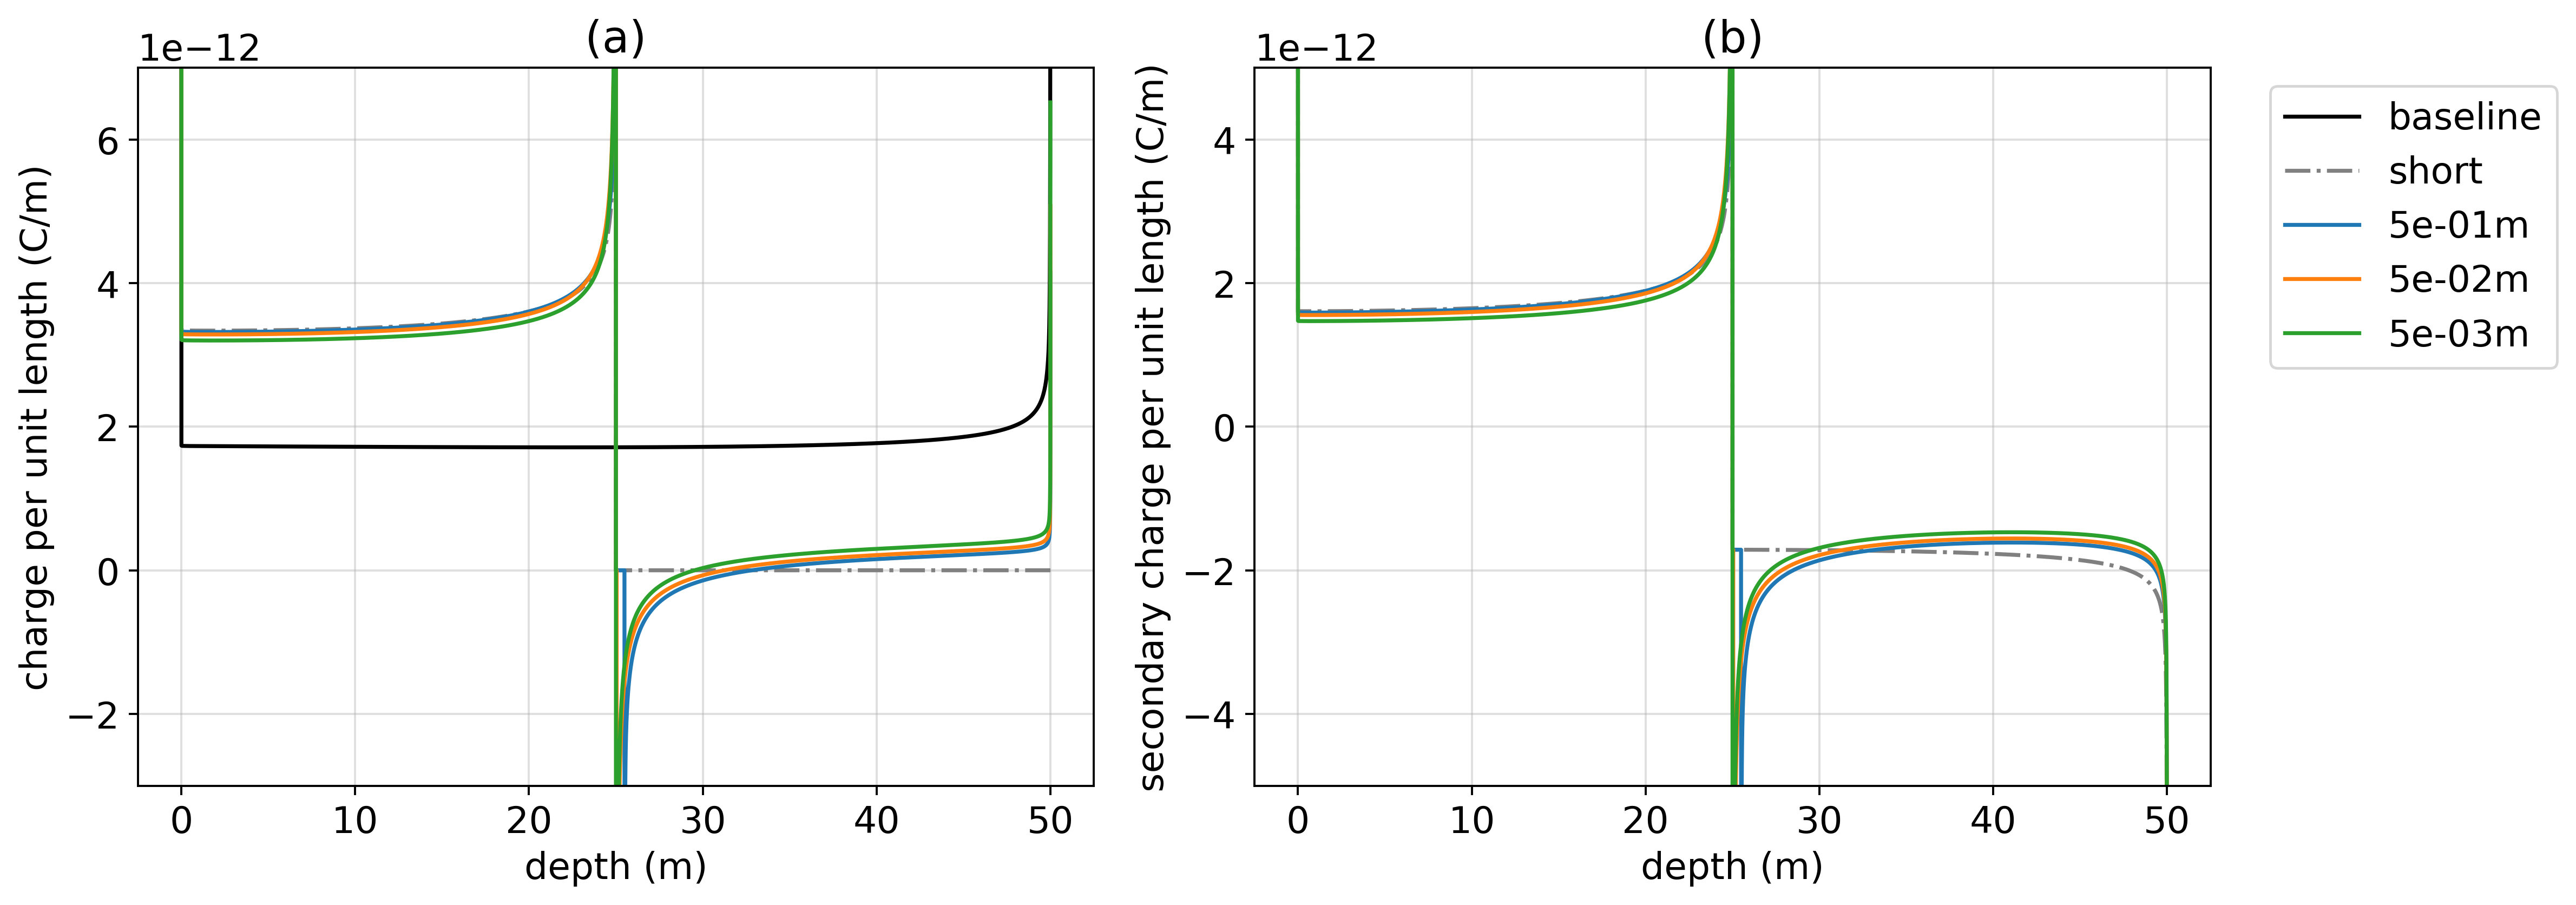
\includegraphics[width=\textwidth]{figures/casing_charge_flawdz.png}
    \end{center}
\caption{
    (a) Charge along the length of a 50m long intact well (black),
    a 25m well (``short'', grey dash-dot), and four wells, each with a flaw
    starting at 25m depth and extending the length indicated by the legend
    ($5 \times 10^{-1}$ m (blue), $5 \times 10^{-2}$ m (orange), and $5 \times 10^{-3}$ m (green))
    in a top-casing DC resistivity experiment.
    For reference, the diameter of the casing is $10^{-1}$ m and its thickness is $10^{-2}$ m.
    (b) Secondary charge along the flawed and short wells. The primary is
    the baseline in (a). The return electrode
    is 50m away from the well and a cylindrically symmetric mesh was used in the simulation.
}
\label{fig:casing_charge_flawdz}
\end{figure}
